\documentclass{standalone}

\usepackage{tikz}

\begin{document}
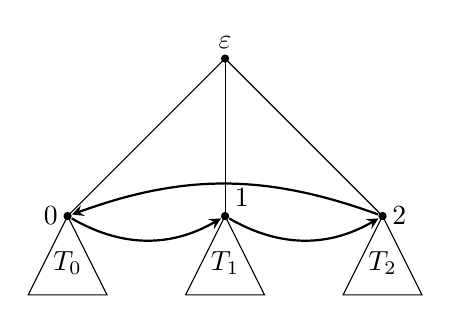
\begin{tikzpicture}[scale=2,>=stealth]

  \fill[black] (1,1) circle (0.1pt) node [above] {$\varepsilon$};
  \fill[black] (0,0) circle (0.1pt) node [left] {$0$};
  \fill[black] (1,0) circle (0.1pt) node [above right] {$1$};
  \fill[black] (2,0) circle (0.1pt) node [right] {$2$};
  
  \node[circle,fill=black,inner sep=0pt,minimum size=3pt] (ID) at (1,1) {};
  \node[circle,fill=black,inner sep=0pt,minimum size=3pt] (T0) at (0,0) {};
  \node[circle,fill=black,inner sep=0pt,minimum size=3pt] (T1) at (1,0) {};
  \node[circle,fill=black,inner sep=0pt,minimum size=3pt] (T2) at (2,0) {}; 
  
  \draw[->,thick] (T0) to [bend right] (T1);
  \draw[->,thick] (T1) to [bend right] (T2);
  \draw[->,thick] (T2) to [bend right=20] (T0);
  
  \draw (1,1) -- (0,0);
  \draw (1,1) -- (1,0);
  \draw (1,1) -- (2,0);
  
  %\draw[->,thick] (0.60,0.55) to (0.95,0.55);
  %\draw[->,thick] (1.05,0.55) to (1.4, 0.55);
  
  %\draw[<-,thick] (0.5,0.475) to [bend right] (1.5,0.475);
  
  \draw[]
    (0,0) -- (0-0.25,-0.5) -- (0+0.25,-0.5) -- cycle;
    
  \draw[]
    (1,0) -- (1-0.25,-0.5) -- (1+0.25,-0.5) -- cycle;
    
  \draw[]
    (2,0) -- (2-0.25,-0.5) -- (2+0.25,-0.5) -- cycle;
    
  \draw[] (0,-0.3) node [] {$T_0$};
  \draw[] (1,-0.3) node [] {$T_1$};
  \draw[] (2,-0.3) node [] {$T_2$};
  
\end{tikzpicture}
\end{document}